
Let $X_1\in\,$\cbrak{2,3,4,5} and $X_2\in\,$\cbrak{11,12,13,14,15} be the random variables such that $X_1$ represents the number chosen from set A and $X_2$ the number chosen from set B.\\
Then, the probability mass functions are 
\begin{align}
    p_{X_1}(n) = \pr{X_1 = n} = 
    \begin{cases}
    \frac{1}{4} & 2 \leq n \leq 5\\
    0 & otherwise
\end{cases}\label{ee2015-2:1}
\end{align}
\begin{align}
    p_{X_2}(n) = \pr{X_2 = n} = 
    \begin{cases}
    \frac{1}{5} & 11 \leq n \leq 15\\
    0 & otherwise
\end{cases}\label{ee2015-2:2}
\end{align}
Let X be the random variable denoting the sum (X=$X_1$+$X_2$). Then, X can take the values \cbrak{13,14,15,16,17,18,19,20}.
\begin{align}
     p_X(n)&=\pr{X_1+X_2=n}\\
     &=\pr{X_1=n-X_2}\\
     &=\Sigma_{k}{\pr{X_1=n-k|X_2=k}p_{X_2}(k)}\label{ee2015-2:3}
\end{align}
 As $X_1,X_2$ are independent,
\begin{align}
    \pr{X_1=n-k|X_2=k}=\pr{X_1=n-k}\label{ee2015-2:4}
\end{align}
from \eqref{ee2015-2:3} and \eqref{ee2015-2:4}
\begin{align}
    p_X(n) = \Sigma_{k} p_{X_1}(n-k)p_{X_2}(n)
    &= p_{X_1}(n)*p_{X_2}(n)\label{ee2015-2:5}
\end{align}
where * denotes the convolution operator.\\
As,
\begin{align}
    p_X(n) &= \Sigma_{k} p_{X_1}(n-k)p_{X_2}(k)\\
    &= \frac{1}{5} \sum_{k=11}^{15}p_{X_1}(n-k)\\
    &= \frac{1}{5} \sum_{k=n-15}^{n-11} p_{X_1}(k)
\end{align}
Since $p_{X_1}(k)=0$ for $k<2 , k>5$\\
Therefore, we get 
\begin{align}
    p_x(n) = 
    \begin{cases}
    0 & n \leq 12\\
    \frac{1}{5} \sum_{k=2}^{n-11}p_{X_1}(k) & 2 \leq n-11 \leq 5\\
    \frac{1}{5} \sum_{k=n-15}^{5}p_{X_1}(k) & 2 \leq n-15 \leq 5\\
    0 & n>20
    \end{cases}
\end{align}
Therefore, from \eqref{ee2015-2:1} we get
\begin{figure}[!hbt]
    \centering
    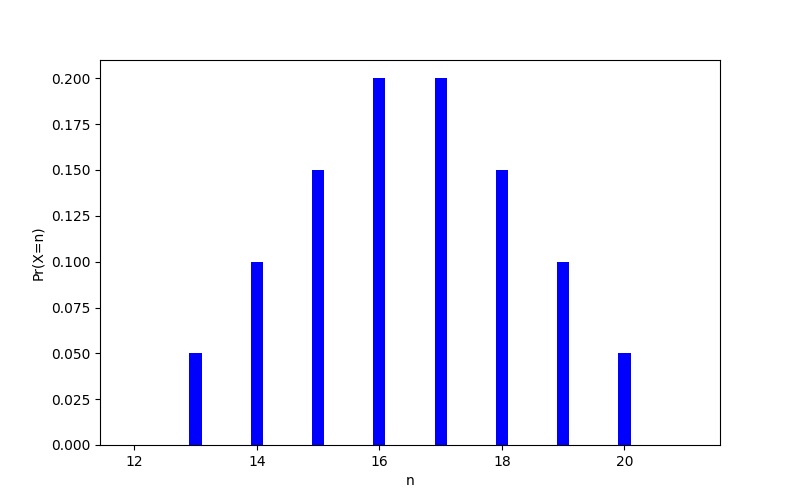
\includegraphics[width=\columnwidth]{solutions/ee/2015/2/Figure_1.png}
    \caption{Probability mass function of X}
    \label{ee2015-2:Figure_1}
\end{figure}
\begin{align}
    p_x(n) = 
    \begin{cases}
    0 & n \leq 12\\
    \frac{n-12}{20}  & 13 \leq n \leq 16\\
    \frac{21-n}{20}  & 17 \leq n \leq 20\\
    0 & n>20
    \end{cases}\label{ee2015-2:6}
\end{align}
Required probability is the probability of the sum of numbers selected from the sets, one from each set to be 16.\\
Therefore from \eqref{ee2015-2:6},
\begin{align}
    p_X(16) &= \left(\frac{16-12}{20}\right)\\
    \implies p_X(16) &= \frac{4}{20}\\
    \implies\pr{X_1+X_2=16} &= \frac{1}{5} \\
    \therefore \pr{X_1+X_2=16}  &= 0.2
\end{align}
